\subsection{共同的图表示与决策空间}
原始输入是一张有向无环的算子--张量图。令 $\mathcal O$ 为操作节点，$\mathcal X$ 为张量节点；张量 $x$ 的生产操作为 $p(x)$，消费操作集合为 $C(x)$，大小为 $b_x$ 字节。原始的 \texttt{COPY\_IN} 与 \texttt{COPY\_OUT} 是既有数据路径，不属于外层切图决策；令 $\mathcal O_c$ 为允许分配子图的其余操作。为讨论依赖，在操作层构造投影弧集合
\begin{equation}\label{eq:op-projection}
E_c=\{(u,v):\exists x\in\mathcal X,\ p(x)=u,\ v\in C(x),\ u,v\in\mathcal O_c\}.
\end{equation}
投影只便于分析，不丢弃张量的身份、字节数及一对多消费关系。若一个输入张量同时供给三个算子，三条投影边仍共享同一个逻辑张量；通信是否发生三次必须由具体场景的 Task 和缓存规则决定。将 $(p(x),C(x))$ 看成有向超边，正是为了避免把共享输入的读入次数误等同于普通割边条数。

对于核数 $k$，方案表示为 $p=(\pi,m,\sigma)$。其中 $\pi:\mathcal O_c\to\{1,\ldots,q\}$ 为非空子图划分，$m:\{1,\ldots,q\}\to\{1,\ldots,k\}$ 为核心映射，$\sigma_c$ 是核心 $c$ 上各子图的排列。若 $\pi(u)\ne\pi(v)$ 且 $(u,v)\in E_c$，则商图有弧 $\pi(u)\to\pi(v)$。核心上的顺序还诱导相邻子图串行弧。令
\begin{equation}\label{eq:expanded-quotient}
H(p)=\bigl(\{1,\ldots,q\},E_\pi\cup E_\sigma\bigr),\quad
E_\pi=\{(\pi(u),\pi(v)):(u,v)\in E_c,\ \pi(u)\ne\pi(v)\}.
\end{equation}
必要合法条件是 $H(p)$ 无环。证明并不只依赖原图无环：即使 $E_\pi$ 无环，错误的核上顺序也可能产生 $A\to B$ 的数据依赖和 $B\to A$ 的串行顺序，形成互等。对每个候选重新拓扑检查 $H(p)$，才能保证至少存在满足先后关系的顺序扩展。图中的任意子图必须非空，且每个可切算子仅出现一次：
\begin{equation}\label{eq:partition-cover}
V_r=\pi^{-1}(r)\ne\varnothing,\qquad
\bigcup_{r=1}^{q}V_r=\mathcal O_c,\qquad
V_r\cap V_s=\varnothing\quad(r\ne s).
\end{equation}
本文不把“每块固定包含若干算子”当作可行性条件；固定块长仅是生成一种候选的启发式参数。任务数、映射和排列均随图结构变化。

这种联合决策的规模解释了为什么必须限制搜索。忽略依赖后，$n=|\mathcal O_c|$ 个带标签算子划成 $q$ 个非空无标签子图已有第二类 Stirling 数 $S(n,q)$ 种，满足
\begin{equation}\label{eq:stirling}
S(n+1,q)=S(n,q-1)+qS(n,q).
\end{equation}
前一项让新算子独立成组，后一项把它加入已有 $q$ 组之一。再为 $q$ 个子图选核心，最多有 $k^q$ 个映射；固定每核的子图集合后，还存在各核排列。依赖和内存约束会删去部分组合，但并不会使“枚举全部划分、核心、次序”在百图规模上可行。因此结构候选只覆盖有依据的局部，官方评价机会在同一预算下分配，而不是对指数空间作均匀遍历。

\subsection{从固定工作量到事件完成时间}
若把每个子图预先赋予一个固定时长，再做普通多机排程，模型会漏掉两层内生变化。其一，外层划分改变核内张量的生存区间，官方核内启发式可能在容量压力下插入换出与换入；于是同一子图放在不同上下文中，展开后的 COPY 与 Pipe 序都可能不同。其二，多个核心的搬运共同占用 DDR，实际传输时长取决于同时在途操作的集合。令 $e$ 为展开后的执行事件，$s_e,f_e$ 为起止时刻，$d_e=f_e-s_e$ 为其实现时长。对固定时长的计算操作，有 $d_e=c_e$；对搬运事件，$d_e$ 由带宽过程产生。发射必须等待它的所有前驱、同一 Pipe 的上一事件和外部释放：
\begin{equation}\label{eq:event-release}
s_e\ge
\max\left\{
\max_{a\in\operatorname{pred}(e)}f_a,\
f_{\operatorname{prevPipe}(e)},\
r_e^{\rm ext}
\right\}.
\end{equation}
上式是依赖约束，尚不是一个可直接把 $d_e$ 相加的显式日程；传输与计算可在不同 Pipe 上重叠。将所有实际事件和资源先后关系构成扩展事件图 $\mathcal H(p)$ 后，在\emph{固定一次仿真已经给出的}搬运时长条件下，完成时间等于源到汇的最长事件路径：
\begin{equation}\label{eq:realized-critical-path}
T(p)=\max_{\gamma\in\Gamma(\mathcal H(p))}
\left(\sum_{e\in\gamma}d_e+
\sum_{(a,e)\in\gamma}\ell_{ae}\right).
\end{equation}
这里 $\ell_{ae}$ 只放路径上真正额外发生的释放等待。不同任务的 DDR 忙碌、计算和同步可能同时发生，不能把全局“DDR 忙碌总时长”“Pipe 空闲总时长”“任务释放等待总时长”直接相加当作可节省周期。诊断必须追问某段等待是否落在最终输出的控制路径上。式\eqref{eq:realized-critical-path}是事后时间线的解释式；因为 $d_e$ 随竞争状态变化，它不是外层优化的线性目标。

共享 DDR 可以按连续时间的服务工作量描述。令 $A_D^+(t)$ 为时刻 $t$ 尚有正剩余工作量的 DDR 搬运集合，事件 $e$ 发射时的独占参考工作量为 $w_e(s_e)=\lceil b_e/B_D\rceil$，其中 $B_D=60$ bytes/cycle。在活跃集合不变的开区间内，公平共享的连续部分满足
\begin{equation}\label{eq:ddr-fluid-common}
\frac{{\rm d}w_e(t)}{{\rm d}t}=-\frac{1}{|A_D^+(t)|},
\qquad e\in A_D^+(t).
\end{equation}
到达或完成事件发生时先结算过去时间段的剩余工作，再重算下一完成事件；最后按官方整数周期与同刻事件次序执行。式\eqref{eq:ddr-fluid-common}解释了为什么只对某个 Task 加上 $b_e/60$ 惩罚不准确：新传输会拖慢同时在途的其他传输，而与其无依赖的 Cube/Vector 计算可能继续。一个候选改变启动时刻后，竞争集合也随之改变，局部估价只能为官方评价筛选候选。

\subsection{可证明下界与诊断的边界}
令 $W_M$、$W_V$ 为原图中矩阵和向量固定周期操作的总工作量，$L_{\rm op}$ 为只计这些操作本身周期的最长依赖链。无论切图怎样安排，在 $k$ 核、每核各一条同类 Pipe 的条件下，都有
\begin{equation}\label{eq:universal-compute-bound}
T_{i,k}\ge L_0(k):=
\max\left\{\frac{W_M}{k},\frac{W_V}{k},L_{\rm op}\right\}.
\end{equation}
工作量项由抽屉原理推出：若所有核心的矩阵 Pipe 占用都小于 $W_M/k$，总占用便小于必须执行的 $W_M$，矛盾；向量 Pipe 同理。最长链项由逐条算子依赖递推，链上计算不能并行。原图固定周期操作不因划分消失，所以式\eqref{eq:universal-compute-bound}对三个问题均适用。它忽略了存储、启动和同步，因而可能很松，但与候选方案无关，可以安全作为统一理论参照。

对\emph{已固定}的方案 $p$，设实际事件展开中 DDR 总搬运字节为 $B_D(p)$。带宽容量再给出一个更强但\emph{方案依赖}的事后界：
\begin{equation}\label{eq:conditional-bandwidth-bound}
T(p)\ge \frac{B_D(p)}{60},
\qquad
L(p)=\max\left\{L_0(k),\frac{B_D(p)}{60}\right\}\le T(p).
\end{equation}
因为 DDR 在一周期内合计最多搬运 $60$ 字节，全部字节即便连续传输也要至少上述时间。$B_D(p)$ 包含原始 COPY、因划分新增的 COPY 和核内溢出；它随 $p$ 改变。因此 $T(p)-L(p)$ 只能描述这个候选相对自身宽松界的松弛，\emph{不能}据此宣称它距所有方案的最优值还有多少。即使差距很小，也可能有另一方案同时显著减少 $B_D$ 和 $T$。对于问题三，还须把 DDR 与 L2 分成两个独立服务池，不能把两条带宽简单相加。

\subsection{两种全量指标的严格区别}
对图 $i$，题目指定整图核内启发式给出固定单核参考时间 $T_{i,1}^{0}$，所交多核方案的时间为 $T_{i,k}$。赛题规定的“平均加速比”是
\begin{equation}\label{eq:mean-speedup-derivation}
\overline S_k=\frac{1}{N}\sum_{i=1}^{N}\frac{T_{i,1}^{0}}{T_{i,k}},
\qquad N=100.
\end{equation}
若关心这一批图合计要占用多少周期，也可报告总周期下降率
\begin{equation}\label{eq:total-reduction}
\rho_k=1-\frac{\sum_iT_{i,k}}{\sum_iT_{i,1}^{0}}.
\end{equation}
二者不是同一统计量。令 $S_{i,k}=T_{i,1}^{0}/T_{i,k}$，则总周期比可改写为
\begin{equation}\label{eq:weighted-speedup}
\frac{\sum_iT_{i,1}^{0}}{\sum_iT_{i,k}}
=\frac{\sum_iT_{i,k}S_{i,k}}{\sum_iT_{i,k}}
=\sum_i\omega_{i,k}S_{i,k},
\quad
\omega_{i,k}=\frac{T_{i,k}}{\sum_jT_{j,k}}.
\end{equation}
所以总周期比是以\emph{多核耗时}为权重的加速比，而式\eqref{eq:mean-speedup-derivation}是每图等权。两个数值可以同时陈述，但不能互换作题目要求的折线图纵轴。若某些大图总周期改善很多、而大量小图改善一般，总周期下降可以明显，平均加速比却不一定同幅增长。后续结果表同时列出平均加速比、百图总周期和额外搬运，正是为了避免单一指标遮蔽这层差异。
图\ref{fig:scene-paths}用相同的依赖关系说明三种场景的服务路径。P、Q、R 表示子图，P 与 Q 同核、R 在另一核心；示意图只说明规则，不表示实测时长。同核驻留仍受依赖与容量约束；共享只读 L2 的命中不取消原有跨核同步。
\begin{figure}[!htbp]\centering
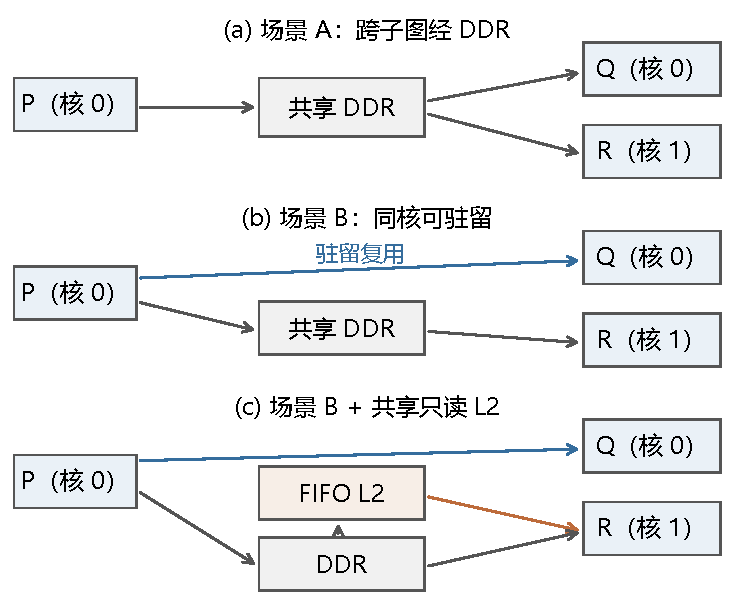
\includegraphics[width=0.92\linewidth,height=0.70\textheight,keepaspectratio]{../图表/runs/20260926-A-six-figures/fig_scene_paths.pdf}
\caption{三种场景的子图数据路径对照}\label{fig:scene-paths}
\end{figure}
